%!TEX root=Principal.tex
\chapter{CLASSIFICADOR BAYESIANO DO USUÁRIO COM BASE NO COMPORTAMENTO DO ROBÔ E HEURÍSTICAS}
\label{cap:proposta}

Nos capítulos anteriores é possível identificar que a existência de robôs em ambientes sociais torna-se cada vez mais comum no dia-a-dia das pessoas. Como qualquer produto existente no mercado, é necessário que os robôs proporcionem uma boa experiência aos usuários durante o uso, que nesse caso é o convívio em ambiente doméstico ou industrial. Entretanto, as técnicas difundidas em interação humano-computador, que tem o objetivo de aumentar a experiência positiva do usuário em produtos tecnológicos, são pouco aplicadas por pesquisadores na área de robótica social, de serviço e assistiva~\cite{alenljung:2017}.

Dado o cenário onde a melhora da interação pode ser alcançada através do uso das técnicas de interação humano-computador, como as voltadas para usabilidade, essa tese apresenta um classificador bayesiano do perfil de usuário. A classificação é feita através das Personas que representam o usuário com base nas ações do robô, informações sobre conforto, desconforto e medo do usuário, técnica de \emph{Proxemics} para compreensão do espaço social e também de informações observadas através das heurísticas de avaliação de interface. O intuito é possibilitar que o robô seja capaz de identificar o perfil do usuário que está interagindo e a partir desse conhecimento consigar tomar a decisão de ações que promovam a melhora do relacionamento entre eles. No futuro, é esperado que o robô possa deixar o usuário a vontade enquanto convivem no mesmo ambiente, como se ele fosse um membro da família.

O trabalho apresentado nessa seção, serve como guia para classificação de usuário durante a interação e aproximação do robô. O uso desse classificador auxilia a identificar o usuário com base na sua experiência de interação com o robô, sendo ela positiva ou negativa. As técnicas utilizadas para compor esse classificador são: (I) Personas, técnica utilizada para representar um grupo de usuários através de um personagem fictício que possui o perfil médio do grupo; (II) Heurísticas de Interação utilizadas para avaliação da interface de um sistema, foram adaptadas para a interação humano-robô. Elas auxiliam o robô a medir variáveis sobre a experiência do usuário na interação; e (III) \emph{Proxemics}, teoria de proximidade (vide seção~\ref{cap:proxemics}), que estuda o comportamento de agentes sociais de acordo com a distância entre si, auxiliando o robô a se posicionar de maneira adequada a uma interação social.

Outro ponto importante apresentado na literatura, é sobre a cultura da pessoa. A cultura influência diretamente o comportamento de uma pessoa em ambientes sociais. Isso significa que algumas reações apresentadas por pessoas no ambiente social são influenciadas pelo seu local de nascimento, pelos locais onde viveu e, consequentemente, pela sua experiência de vida. Fatores como a experiência de vida e cultura são difíceis de avaliar apenas através da observação. Conseguir fazer com que uma pessoa tenha liberdade para contar esse tipo de informação necessita de interações de longo prazo, podendo levar meses até compreender toda história dessa pessoa. Algumas questões referentes a cultura do usuário são discutidas nos resultados apresentados no capítulo~\ref{cap:resultados}.

Sendo o robô um produto tecnológico, é importante o uso de técnicas que sejam capazes de aumentar a efetividade da interação, não havendo a necessidade de conhecer por completo a história de vida do indivíduo em questão. Essas técnicas tem o objetivo de deixar o sistema mais fácil de usar e acima de tudo aumentar a experiência, a satisfação do usuário ao utilizá-lo. Para que o robô possa realizar essa classificação e raciocínio sobre as informações que existem no ambiente alguns passos são apresentados ao longo deste capítulo.

Com base no robô disponível para os experimentos, as ações que são possíveis para ele executar são estabelecidas. A seção~\ref{sec:robo} apresenta em detalhes o robô utilizado para essa pesquisa. Na sequência dois questionários são apresentados, o primeiro aplicado antes do teste de interação e o segundo após. O primeiro questionário estabelece o perfil do usuário referente a questões de aderência a tecnologia, contato prévio com robôs, a cultura que ele se identifica e a expectativa em relação a robôs em ambientes domésticos e profissionais. O questionário pós-teste possui informações declaradas sobre o conforto, desconforto, medo e avaliação do comportamento do robô, durante a interação.

Após definição dos questionários, 39 pessoas foram selecionadas para participar do teste de interação com o robô, de acordo com o cenário descrito na seção~\ref{sec:cenario}. Os testes foram executados com o comportamento do robô de maneira aleatória, ou seja, com o mínimo de preocupação com a experiência do usuário neste momento, apenas zelando pela segurança. Coletados os perfis e informações dos usuários, é realizado uma preparação e normalização dos dados para que o algoritmo QG-SIM possa realizar o agrupamento dos perfis similares, conforme o processo apresentado por \citeonline{masiero:2013b}. A partir dos grupos gerados pelo algoritmo QG-SIM, é realizado o processo de criação de Personas~\cite{masiero:2013, masiero:2013b}.

Personas são criadas com base nas informações extraídas de cada grupo através dos questionários de pré e pós teste de interação. O próximo passo, é estabelecer as dependências condicionais entre cada variável aleatória incluida através da análise dos dados e observações dos testes de interação. As variáveis são compostas pelas Personas criadas, algumas heurísticas que se enquadram nas observações realizadas pelos usuários durante a interação com o robô, a proximidade entre robô e usuário que é importante para identificar os comportamentos e reações dado o espaço social ocupado, as ações e comportamentos do robô e efeitos de conforto, desconforto e medo da pessoa durante a interação. Essa dependência condicional entre as variáveis faz com que elas sejam organizadas no formato de uma rede bayesiana. O objetivo dessa rede é classificar qual o perfil do usuário dado que houve a leitura de conforto, desconforto e/ou medo durante a interação com o robô em um cenário residencial.

As variáveis aleatórias foram definidas de maneira abstrata e podem, no futuro, sugir outras que auxiliem na classificação do usuário de maneira que o resultado da rede bayesiana possa servir como alimentação de um mecanismo de decisão do robô para melhorar a interação com o usuário. Ao final, um conjunto de variáveis são propostos como pontos para futuras investigações e evolução do classificador entregue por essa tese.

\section{Ações e Comportamentos do Robô}
\label{sec:comportamento-robo}
O robô escolhido para os experimentos possui uma série de características que auxiliam a interação social e serviço domésticos, uma vez que ele foi construído para atender a competição de robótica RoboCup@Home~\cite{robocup:2015}. Com base nos atuadores de interação existentes (vide seção~\ref{sec:robo}), foram mapeados as variáveis de ações e comportamentos do robô. A tabela~\ref{tab:variaveisvalores} apresenta as variáveis, compostas por seus respectivos valores.

\begin{table}[!ht]
	\caption{Variáveis de Comportamento do Robô}
	\label{tab:variaveisvalores}
	\centering
	\begin{tabular}{c | c}
		\hline
		Variável & Valor \\
		\hline
		Gestos & curto \\
		& longo \\
		\hline
		Estilo da Fala & educada \\
		& autoritária \\
		\hline
		Expressão Facial & amigável \\
		& não amigável \\
		\hline
		Proximidade & longe - (Entre Pública e Social ) \\
		& perto - (Entre Pessoal e Íntima ) \\
		\hline
		Velocidade & rápida \\
		& devagar \\
		\hline
		Posição & sentado \\
		& em pé \\
		\hline
	\end{tabular}
	\smallcaption{Fonte: O autor.}
\end{table}

Além das variáveis direcionadas aos atuadores do robô, a tabela~\ref{tab:variaveisvalores} apresenta a variável de proximidade entre o robô e o ser humano e a variável posição que determina como o usuário estava durante a interação, sentado ou em pé. São variáveis importantes, pois auxiliam a determinar o comportamento de reação da pessoa para um mesmo tipo de gesto do robô em diferentes situações. Por exemplo, se o robô encontra-se próximo da pessoa, entre as zonas Pessoal e Íntima, um gesto amplo pode gerar um desconforto maior do que o mesmo gesto ocorrendo entre as zonas Pública e Social. Ou como é a reação do usuário quando o robô aproximar o manipulador próximo ao rosto do usuário.  A partir das variáveis definidas e comportamentos implementados no robô é importante agora trabalhar com os questionários pré e pós testes.

\section{Questionários para Coleta de Dados de Interação}
\label{sec:questionarios}
Para apoiar o processo de obtenção das informações e construção dos perfis dos usuários, dois questionários foram construídos. O primeiro, aplicado no momento anterior ao experimento de interação, tem como objetivo mapear as informações referentes às características físicas que tem a possibilidade do robô utilizar sensores para reconhecê-las, adesão a tecnologia, contatos prévios com robôs, questões culturais onde o usuário declara quais locais ele possui mais afinidade e quais ele já teve o privilégio de visitar, além da expectativa de possuir um robô em casa ou no trabalho. As questões serão agrupadas de acordo com seus objetivos e apresentadas em listas. Todas as questões a seguir fazem para do questionário pré-experimento.

Questões focadas na identificação e características físicas do usuário:

\begin{enumerate}
	\item Informe seu nome completo
	\item e-mail para contato
	\item Informe o número do seu celular
	\item Testes poderão ocorrer usando o Robô no Centro Universitário FEI. Você gostaria de realizar o teste com o robô físico? Opções de resposta: Sim, Não
	\item Qual a sua idade? (em anos)
	\item Qual a sua altura? (em metros)
	\item Informa seu gênero: Opções de resposta: Feminino, Masculino, Prefiro não dizer
	\item Na maior parte do tempo, você se considera uma pessoa com feição: Opções de reposta: Sorridente, Normal, Séria/Fechada
	\item Você se considera uma pessoa sociável? Opções de resposta: Sim, Não
	\item Você utiliza óculos de grau? Opções de resposta: Sim, Não (Obs: Pessoas com lente de contato, por favor, repondam não. A intenção é identificar a armação.)
	\item Você possui cabelo comprido? Opções de resposta: Sim, Não
	\item Qual etnia você se considera? Opções de resposta: Amarela, Branca, Indígena, Parda, Preta, Não declarada
\end{enumerate}

Questões para informações sobre adesão à tecnologia:

\begin{enumerate}
	\item Qual(is) dispositivo(s) tecnológico(s) você mais utiliza (marque 1 ou mais opções): Opções de resposta: Celular, Computador (de mesa ou notebook), Tablet, Smart TV, Relógio Smart, MP3 Player, Câmera Fotográfica Digital, Leitor de e-Book, outros
	\item Qual(is) dispositivo(s) tecnológico(s) você nunca utilizou (marque 1 ou mais opções): Opções de resposta: Celular, Computador (de mesa ou notebook), Tablet, Smart TV, Relógio Smart, MP3 Player, Câmera Fotográfica Digital, Leitor de e-Book, Já utilizei todas
	\item Você possui conta em banco digital (ex: Original, Neon, etc.) ? Opções de resposta: Sim, Não
	\item Você possui cartão de crédito digital (ex: Nubank, Digio, etc.) ? Opções de resposta: Sim, Não
	\item Qual o principal meio de pagamento de suas contas? Opções de resposta: Celular, Computador, Tablet, Autoatendimento, Caixa Físico
	\item Você utiliza redes sociais? Opções de resposta: Sim, Não
	\item Quais as redes sociais que você mais utiliza (marque 1 ou mais opções): Opções de resposta: Facebook, Instagram, Twitter, Google\+, Snapchat, outras
\end{enumerate}

Questões sobre informações culturais:

\begin{enumerate}
	\item Qual foi o local de nascimento? (Informe da seguinte maneira: Cidade; Estado; País)
	\item Em qual local, você viveu por mais tempo durante sua infância e adolescência? (Informe da seguinte maneira: Cidade; Estado; País)
	\item Qual o seu atual local de moradia? (Informe da seguinte maneira: Cidade; Estado; País)
	\item Qual o país que você melhor se identifica com a cultura? (Considere também a opção do seu país de nascimento.)
	\item Qual a cidade, na sua opinião, que melhor representa a cultura que você se identifica (resposta não dependente da questão acima)?
	\item Você visitou outros países, além do Brasil? Opções de resposta: Sim, Não
	\item Quais países você já visitou? (Responda separando os países por ponto e vírgula, ex: França; Estados Unidos; Itália; Japão;)
	\item Aproximadamente, quantas cidades na região nordeste do Brasil você visitou?
	\item Aproximadamente, quantas cidades na região norte do Brasil você visitou?
	\item Aproximadamente, quantas cidades na região centro-oeste do Brasil você visitou?
	\item Aproximadamente, quantas cidades na região sudeste do Brasil você visitou?
	\item Aproximadamente, quantas cidades na região sul do Brasil você visitou?
\end{enumerate}

Por fim, questões sobre contato prévio com robôs e expectativa de tê-los no trabalho e também em casa:

\begin{enumerate}
	\item Em algum momento de sua vida, você teve contato com robôs? Opções de resposta: Sim, Não
	\item Se sim para a questão anterior, quais tipos de robôs você teve contato (marque 1 ou mais opções): Opções de resposta: Parecido com animais, Parecido com pessoas, Robôs de linha de produção/fábrica, Robôs Móveis (que contém rodas), outros
	\item O que você espera do comportamento do Robô ao tê-lo em sua casa?
	\item O que você espera do comportamento do Robô ao tê-lo em seu trabalho?
	\item Dadas as questões anteriores, gostaria de fazer mais algum comentário sobre você?
\end{enumerate}

O segundo questionário mantém o foco na interação do usuário durante o experimento e quais pontos do robô mais agradaram ou não na opinião dele. Além disso, um detalhe sobre a posição do usuário durante o experimento (sentado ou em pé) é coleta, pois está informação pode influenciar na interação com o robô. As questões apresentas a seguir compõe o questionário pós-teste:

\begin{enumerate}
	\item Informe o número de amostra (Identificador dos documentos referentes ao comitê de ética)
	\item Você se sentiu confortável durante a aproximação do robô? Escala de 1 à 10
	\item Você se sentiu com medo em algum momento durante a aproximação do robô? Escala de 1 à 10
	\item Você estava \_\_\_\_\_\_\_\_\_ durante a aproximação do robô. Opções de resposta: Sentado, em Pé
	\item Você voltaria a interagir com esse robô novamente? Opções de resposta: Sim, Não
	\item Justifique a resposta anterior.
	\item O que você mais gostou no robô?
	\item O que você menos gostou no robô?
	\item Depois dessa experiência, você interagiria com outros robôs? Opções de resposta: Sim, Não
	\item Você estaria confortável com um robô convivendo em sua casa? Opções de resposta: Sim, Não
	\item Justifique a resposta anterior.
	\item Em algum momento da interação, você se sentiu desconfortável com o comportamento do robô? Opções de resposta: Sim, Não
	\item Descreva o desconforto em caso de sim, na resposta anterior.
	\item Você alteraria algum comportamento apresentado pelo robô durante o teste? Qual?
	\item Observações e comentários:
\end{enumerate}

As informações coletadas através dos questionários apresentados são utilizadas no processo de definição das probabilidades referentes as tabelas condicionais das variáveis aleatórias que compõem a rede bayesiana. Todo o processo e questionários apresentados nesse capítulo são aprovados pelo comitê ética sobre identificador de processo CAAE: 70057117.0.0000.5508.

\section{Preparando os dados para o algoritmo QG-SIM}
\label{sec:preparacao}
Com as informações obtidas através dos testes e observações das interações, é necessário trabalhar na normalização dos dados para que seja possível executar o algoritmo que agrupará os perfis semelhantes. Nesse momento, é necessário uma análise manual para separar as informações. O primeiro passo é deixá-las todas em uma única base de dados, pois encontram-se em bases distintas.

Base de dados unificada, o próximo passo é remover as informações de texto livre, uma vez que o algoritmo não possui um interpretador semântico e dessa maneira não é possível criar um modelo quantitativo para essas respostas, de maneira que exista uma significância comparativa entre as respostas.

As informações quantitativas existentes, como por exemplo a idade do usuário, pode-se aplicar medidas como a distância euclidiana para realizar a comparação entre um perfil e outro. Outras medidas também podem ser aplicadas, isso fica a critério da necessidade do projeto~\cite{masiero:2013}. No caso do agrupamento de perfis desta tese, a distância euclidiana é adotada já que atende a necessidade do algoritmo e do processo para agrupamento dos perfis.

Em relação as variáveis categóricas, ou seja, as variáveis que possuem um valor textual que podem ser separadas por categoria, existem duas opções para converte-las em valores quantitativos. A primeira opção é inserir um código númerico para cada valor, por exemplo, os valores ``Celular, Computador, Tablet, Autoatendimento, Caixa Físico'' recebem um valor representado por um número inteiro cada ficando ``Celular = 1, Computador = 2, Tablet = 3, Autoatendimento = 4, Caixa Físico = 5'', conforme~\citeonline{masiero:2013}. A segunda opção é transformá-las em variáveis \emph{dummies}~\footnote{http://pandas.pydata.org/}. O método \emph{dummies} transforma cada opção de resposta ou cada categoria em uma nova variável binária onde o valor 1 é para quando a opção for verdadeira e 0 para o oposto.

Nesse ponto a base de dados está com todas as variáveis quantificadas, porém existe um segundo problema que pode afetar o resultado do algoritmo. Cada variável possui uma escala diferente. Essa diferença na escala das variáveis pode gerar tendências no resultado do algoritmo, assim é necessário padronizar os valores númericos existentes na base. Para realizar a padronização dos dados o processo de normalização é executado. A normalização mais comum a ser feita é manter os valores das variáveis entre 0 e 1~\cite{lattin:2011}. A equação~\ref{eq:normalizacao1} apresenta a forma mais simples de realizar o processo de normalização dos dados. É feita a divisão do valor da característica pelo valor máximo encontrado entre a característica analisada.

\begin{equation}
	X_{i_{normalizado}} = \frac{X_i}{\max_{X_i}}
	\label{eq:normalizacao1}
\end{equation}

Entretanto, o uso da equação \ref{eq:normalizacao1} para normalizar os dados, pode gerar também uma tendência ou generalização da normalização. Pode existir uma concentração dos dados em um determinado intervalo generalizando a informação coletada~\cite{masiero:2013}. Para evitar o problema da concentração dos dados, utiliza-se a equação \ref{eq:normalizacao2} como método mais efetivo na normalização dos dados.

\begin{equation}
	X_{i_{normalizado}} = \frac{X_i - \min_{X_i}}{\max_{X_i} - \min_{X_i}}
	\label{eq:normalizacao2}
\end{equation}

Após o processo de normalização, as escalas da base estão com uma distribuição uniforme e prontas para serem consumidas pelo algoritmo.

\section{Executando o QG-SIM e criando as Personas}
\label{sec:criarpersonas}
Com as informações normalizadas, o próximo passo é executar o algoritmo de agrupamento QG-SIM. A implementação do algoritmo pode ser encontrada no endereço \url{https://github.com/amasiero/qgsim}. O algoritmo solicita um valor de similaridade mínimo para manter a qualidade entre os elementos de um mesmo grupo. Esse valor é chamado de Q. A partir desse valor, o QG-SIM agrupará os perfis de acordo com a similaridade desejada e o número de grupos é obtido automaticamente através do valor Q~\cite{masiero:2013}.

Assim que os grupos são definidos, é necessário encontrar a medida de dispersão central para cada uma das variáveis do perfil. As medidas de dispersão mais comuns são: média, mediana e moda. Elas auxiliam no processo de construção da Persona, como definição de idade, o uso de óculos, tipo do cabelo, gênero, e outras informações. Como os grupos encontrados não possuiam ruídos em sua distribuição, a medida de disperção adota foi a média (vide capítulo~\ref{cap:resultados}). Nesse momento, as informações de texto livres preenchidas são utilizadas para análise que é base para preencher a descrição e história da Persona. É verificado cada resposta dos indivíduos que compõe o grupo e na sequência é criado toda uma história de vida e experiências para a Persona.

Nesse processo, cinco Personas foram encontradas e são apresentadas a seguir:
\begin{table}[!ht]
	\caption{Persona Joaquim}
	\label{tab:joaquim}
	\centering
	\begin{tabular}{ m{2 cm} | m{13cm} }
		\hline
		Foto: & \rule{0cm}{2.7cm} 
\includegraphics[scale=0.8]{joaquim.png} \\
		\hline
		Nome: & Joaquim \\
		\hline
		Descrição: & Tem 21 anos, 1,71 m de altura, em geral não é uma pessoa séria ou carrancuda, mas também não é sorridente. É um homem sociável, cheio de amigos a sua volta e adora ir ao barzinho com eles. Mora na capital paulista, centro econômico brasileiro, local perfeito para um homem que gosta de variedade cultural. Não fica longe de seu smartphone e também sempre que pode, está com seu laptop no colo navegando pelo Facebook e postando fotos no Instagram. Tudo que pode ser resolvido pelo seu smartphone ele faz, seja por chamada de voz ou qualquer aplicativo. Mas, ainda não conseguiu se habituar aos serviços financeiros digitais, prefere o método clássico para guardar seu dinheiro, o colchão. Nunca viajou para fora do Brasil, inclusive seu mapa de viagens nacionais também não é extenso. Ao todo, visitou apenas 9 cidades do Brasil com o passar do tempo.

		Na universidade acompanhou os times de robótica nas competições e teve contato com diversos tipos de robôs, como os parecidos com humanos e animais, com mobilidade através de rodas e também os de linha de produção. Quando perguntam sua expectativa sobre robôs convivendo em sua casa, ele diz que tudo bem, desde que ele execute as tarefas domésticas sempre com obediência e de certa maneira, também espera que o robô seja afetivo na interação. Um comportamento próximo ao de uma diarista na família. Já no ambiente industrial, Joaquim acredita que os robôs são apenas ferramentas de trabalho e não devem fazer nada além de executar o que lhe foi programado. \\
		\hline
	\end{tabular}
	\smallcaption{Fonte: O autor.}
\end{table}

\begin{table}[!ht]
	\caption{Persona Maria Eduarda}
	\label{tab:mariaeduarda}
	\centering
	\begin{tabular}{ m{2 cm} | m{13cm} }
		\hline
		Foto: & \rule{0cm}{2.7cm} 
\includegraphics[scale=0.8]{maria_eduarda.png} \\
		\hline
		Nome: & Maria Eduarda \\
		\hline
		Descrição: & Aos 36 anos, com 1,71 m de altura, é uma garota reservada que adora sorrir em diversas ocasiões. É bem sociável, e mantém os amigos por perto. É uma mulher moderna e gosta de manter seu corte de cabelo mais curto que o convencional. Mora em São Bernardo do Campo, cidade da grande São Paulo e gosta muito de visitar o interior de São Paulo para passar seus feriados prolongados. Não vive sem seu celular, e no trabalho o computador é sua principal ferramenta. Quando está em casa utiliza sua Smart TV para assistir suas séries e filmes favoritos. Gostario muito de ter um leitor de e-book para evitar carregar livros pesados durante seu trajeto pelo transporte público. Mesmo com essa adoção a tecnologia, empresas digitais, principalmente do mercado financeiro, não a atraem. Sempre conectada através do celular, ela posta tudo no Facebook, tanto de trabalho quanto de lazer.

		Já viajou algumas vezes para os EUA, sempre a passeio com o principal destino a Disney. Pelo Brasil, já viajou para algumas cidades fora de São Paulo e deixou sua marca por todas as regiões do país. Como ela trabalha em uma universidade de engenharia, já viu diversos tipos de robôs, que são utilizados nas aulas. Porém, nunca teve um contato direto com eles, a não ser seu aspirador de pó. Tanto em casa quanto no trabalho, ela espera que robôs sejam capazes de realizar tarefas com eficácia, como dirigir um carro, digitar planilhas, mas que ao mesmo tempo não seja capaz de substituí-la.\\
		\hline
	\end{tabular}
	\smallcaption{Fonte: O autor.}
\end{table}

\begin{table}[!ht]
	\caption{Persona Alfredo}
	\label{tab:alfredo}
	\centering
	\begin{tabular}{ m{2 cm} | m{13cm} }
		\hline
		Foto: & \rule{0cm}{2.7cm} 
\includegraphics[scale=0.8]{alfredo.png} \\
		\hline
		Nome: & Alfredo \\
		\hline
		Descrição: & Aos 24 anos, rapaz de estatura normal, por volta de 1,75m, está sempre com um belo sorriso no rosto, faça chuva ou faça sol. Sempre tem pessoas a sua volta, gosta de contar piadas e fazer todos sorrirem. Morador da cidade de São Bernardo do Campo, mas sempre que pode vai para o litoral paulista visitar os pais e curtir uma praia. Usa computador para fazer os trabalhos da faculdade e passa grande parte do seu tempo no celular. Não possui serviços financeiros digitas, pois ainda não conseguiu a aprovação do cadastro. Quando se trata de internet banking, acredita que o seu computador é mais seguro que o uso de celular.

		Alfredo vive antenado nas redes sociais, como Twitter, Instagram e Facebook. Ajudam ele a ficar conectado com as últimas notícias e eventos a sua volta. Tem um sonho de viajar para o exterior, mas isso ainda não foi possível, em compensação pelo Brasil já visitou mais de 30 cidades, a maioria na região Sudeste. Na universidade, através do curso de engenharia de automação, teve contato com robôs de fábrica e móveis conforme os laboratórios das disciplinas ocorriam. Qunado perguntam a Alfredo o que ele espera de um robô doméstico e também um robô no trabalho, ele diz que robôs devem executar as tarefas propostas de maneira eficiente e que seu interação seja toda por comando de voz.\\
		\hline
	\end{tabular}
	\smallcaption{Fonte: O autor.}
\end{table}

\begin{table}[!ht]
	\caption{Persona Danielo}
	\label{tab:danielo}
	\centering
	\begin{tabular}{ m{2 cm} | m{13cm} }
		\hline
		Foto: & \rule{0cm}{2.7cm} 
\includegraphics[scale=0.8]{danielo.png} \\
		\hline
		Nome: & Danielo \\
		\hline
		Descrição: & Com 27 anos de idade, 1,83m, Danielo está sempre na academia para treinar com seus amigos. Mora em São Bernardo do Campo, e utiliza seu computador para fazer seu trabalho e o celular para manter contato com seus amigos. Nunca quis saber de leitores de e-book, pois acha sua tecnologia sem utilidade nos dias atuais. A sua única rede social é o Facebook. Ele acha que já toma tempo o suficiente e não precisa de outras para ver a mesma coisa. Danielo é um rapaz que já viajou bastante. Já visitou 3 países latinos e no Brasil visitou mais de 90 cidades, concetradas em sua grande parte, na região Sudeste. O contato com robôs é limitado e restrito a robôs de fábrica. Em casa ele acredita que o robô será parecido com seres humanos para fazer as atividades domésticas, e no trabalho substituirão seres humanos em trabalhos repetitivos, como nas fábricas e linha de produção.\\
		\hline
	\end{tabular}
	\smallcaption{Fonte: O autor.}
\end{table}

\begin{table}[!ht]
	\caption{Persona Manuel}
	\label{tab:manuel}
	\centering
	\begin{tabular}{ m{2 cm} | m{13cm} }
		\hline
		Foto: & \rule{0cm}{2.7cm} 
\includegraphics[scale=0.8]{manuel.png} \\
		\hline
		Nome: & Manuel \\
		\hline
		Descrição: & Aos 33 anos, 1,85 m,  Manuel um professor universitário sempre sorridente. Seus alunos sempre o procuram para esclarecer dúvidas e pedir conselhos. Mora em São Bernardo do Campo, próximo ao seu local de trabalho, por que adora o conforto de ir em sua casa poder almoçar uma comida fresca. Acredita que tem uma melhor qualidade de vida assim. Não é muito fã de tecnologia de ponta, então fica contente em ter seu computador, onde resolve tudo que pode. Digitalmente, considera-se antisocial e não mantém cadastro em nenhuma rede social.

		Já visitou paises pela Europa, África, América do Norte e do Sul. No Brasil, seu foco de visitar está na região Sudeste, principalmente o estado de Minas Gerais. No total já percorreu mais de 62 cidades pelo país. Como professor, sua linha linha de pesquisa principal de estudos é a robótica, fazendo com que tenha contato com todos os tipos de robôs. Em casa, pensa em ter um robô para atender suas necessidades, assim como no trabalho. Porém, o robô no trabalho deve atender também as necessidades e expectativas da empresa.\\
		\hline
	\end{tabular}
	\smallcaption{Fonte: O autor.}
\end{table}

As Personas apresentadas nas tabelas~\ref{tab:joaquim}, \ref{tab:mariaeduarda}, \ref{tab:alfredo}, \ref{tab:danielo}, \ref{tab:manuel} foram criadas com base nas informações coletadas nos questionários e ajudaram na definição das independências condicionais da rede bayesiana. Mais informações das análises feitas com base nas Personas, e também sobre sua criação, em relação a interação com o robô são apresentadas no capítulo~\ref{cap:resultados}.

\section{Heurísticas de Interação Humano-Robô}
\label{sec:heuristicas}
Avaliação heurística é um método utilizado por especialistas em usabilidade para verificar problemas de interação em interfaces de sistemas e produtos. \citeonline{nielsen:1994} apresenta 10 heurísticas para avaliações de interfaces em sistemas web (vide seção~\ref{sec:avaliacao}). As heurísticas de Nielsen tem sido amplamente utilizadas ao longo dos tempos para sites e sistemas desktop. Alguns trabalhos apresentados ao longo da seção~\ref{sec:ihrux} apresentam modificações das heurísticas de Nielsen para o cenário de interação humano-robô. Para os fins dessa tese, as heurísticas adaptadas que apresentam uma maior aplicabilidade em robótica social e interação humano-robô são as heurísticas de \citeonline{clarkson:2007}. As heurísticas são apresentadas na tabela~\ref{tab:heuristicasihr}.

Heurísticas de interação e interface são sempre utilizadas com o propósito de avaliar o produto para que o usuário fique mais satisfeito. Porém, durante os primeiros testes de interação entre o robô e o usuário, observou-se que muitas das pontuações sobre conforto, desconforto e até medo estavam dentro das diretrizes das heurísticas. Um ponto importante é que alguns perfis se atentaram a algumas características enquanto outros perfis nem mencionaram isso. Dessa maneira, essa tese propõem o uso das heurísticas como um conjunto de variáveis que complementa a classificação do perfil do usuário. O uso das heurísticas dessa maneria, está alinhada com o conceito de utilidade apresentado na seção~\ref{sec:raciocinio-probabilistico}, onde uma heurística pode ser mais útil para um determinado perfil de usuário do que para um terceiro.

Com base nas observações e informações dos testes de interação foi possível identificar as seguintes heurísticas para uso como variável de classificação do usuário:

\begin{itemize}
	\item Heurística 02: Visibilidade do estado do sistema;
	\item Heurística 04: Uso de sugestões naturais;
	\item Heurística 05: Síntese do sistema e interface;
	\item Heurística 06: Ajudar o usuário a reconhecer, diagnosticar, e recuperar de erros.
\end{itemize}

Cada uma das heurísticas apresentadas na lista acima, foram observadas entre os testes e possuem dependência condicional com os perfis e/ou com as ações do robô. Mais detalhes são apresentados na seção~\ref{sec:rede-bayesiana}, a seguir.

\section{Classificação do Usuário através da Rede Bayesiana}
\label{sec:rede-bayesiana}

Com todos os passos necessários para identificar o usuário e suas necessidades com o projeto, o próximo passo é a criação de um mecanismo que possa fazer com que o robô realize a classificação do perfil do usuário a partir das observações de conforto, desconforto e medo. Tais informações geram incertezas, que podem ocorrer baseadas em falhas de sensores, ruído da percepção do robô perante a ação/reação do usuário, cenário de atuação, estado emocional interno do usuário, entre outros. Dado esse cenário de incerteza, é importante que a técnica utilizada não afirme sobre uma classificação, mas sim possa inferir a probabilidade de uma resposta coerente a sua leitura. Como apresentado na seção~\ref{sec:cbrw}, a técnica de rede bayesiana tem sido utilizada em muitos trabalhos com o mesmo objetivo. Sendo assim, essa seção apresenta uma rede bayesiana que seja capaz de classificar o perfil do usuário com base na informação de conforto, desconforto e medo declarado pelo usuário. Na sequência será apresentado cada conjunto de nós e suas dependências condicionais para a criação da estrutura da rede bayesiana de classificação.

Os nós raizes da rede bayesiana são compostos pelas 5 Personas apresentadas na seção~\ref{sec:criarpersonas}. Elas são escolhidas como raiz por que representam os perfis de usuários que devem ser classificados durante a aproximação do robô para interação. Cada vez que novas interações ocorrem, é possível que novos perfis sejam incluídos para a classificação. A probabilidade do usuário em interação ser ou não aquela Persona é determinada, a princípio, pela quantidade de pessoas que ajudaram a compor ela. Como são nós raizes, não existem nenhuma observação que auxilie na composição do seu valor de probabilidade. As equações~\ref{eq:joaquim}, \ref{eq:mariaeduarda}, \ref{eq:alfredo}, \ref{eq:danielo} e \ref{eq:manuel} representam a probabilidade de cada uma das Personas obtidas.

\begin{equation}
	\label{eq:joaquim}
	P(joaquim)
\end{equation}

\begin{equation}
	\label{eq:mariaeduarda}
	P(maria\_eduarda)
\end{equation}

\begin{equation}
	\label{eq:alfredo}
	P(alfredo)
\end{equation}

\begin{equation}
	\label{eq:danielo}
	P(danielo)
\end{equation}

\begin{equation}
	\label{eq:manuel}
	P(manuel)
\end{equation}

As variáveis são nomeadas com letras minúsculas, pois são variáveis com apenas dois valores representando ser ou não ser. Essa notação segue a convenção apresentada por \citeonline{russell:2002}.

Seguindo com a construção da rede, cada nó interno foi considerado com base nas observações feitas pelos usuários dos testes iniciais. Do mesmo modo que as independências condicionais entre cada nó. A seguir o processo de criação dos nós será detalhado. Os primeiros nós inseridos na camada interna da rede bayesiana foram os comportamentos e ações do robô e também a questão da proximidade e posição do usuário no ambiente, como apresentado na tabela~\ref{tab:variaveisvalores}.

O primeiro nó é o nó Proximidade, que leva em consideração os espaços sociais definidos por \citeonline{hall:1969}. O domínio foi simplificado para \{perto, longe\}, pois durante os testes pilotos a reação do usuário era a mesma entre as regiões íntima e pessoal (perto) e as regiões social e pública (longe). A dependência condicional foi aplicada de acordo com a declaração explícita entre os perfis que sentiram algum desconforto com a aproximação do robô. A equação~\ref{eq:proximidade} define o cálculo de probabilidade condicional para a variável aleatória Proximidade.

\begin{equation}
	\label{eq:proximidade}
	P(Proximidade | joaquim, alfredo, danielo)
\end{equation}

A próxima variável aleatória inserida é a Posição da pessoa no ambiente. O domínio dessa variável é determinado por \{sentado, em pé\}. Ela foi observada durante a prova de reconhecimento de pessoas e aproximação do robô na RoboCup de 2016. Nesse cenário, as pessoas que estavam sentadas ficavam bem desconfortáveis com a aproximação do robô, principalmente com relação ao seu manipulador. Nos teste pilotos, a situação demonstrou-se a mesma. As pessoas que estavam sentadas demonstravam um comportamento mais apreensivo do que as em pé. A equação~\ref{eq:posicao} apresenta o cálculo de probabilidade condicional para a variável Posicao.

\begin{equation}
	\label{eq:posicao}
	P(Posicao | joaquim, maria\_eduarda, alfredo, danielo, manuel)
\end{equation}

As 4 próximas variáveis aleatórias descritas são referentes a ações do robô. Todas os 4 conjuntos são importantes na interação social e geram diferentes reações aos perfis de usuários. Um ponto interessante a ser resaltado é que cada Persona mapeada, ficou atenta durante a interação em apenas algumas das variáveis. As 4 variáveis são Expressão Facial (equação~\ref{eq:face}), Gestos (equação~\ref{eq:gestos}), Estilo da Fala (equação~\ref{eq:fala}) e Velocidade (equação~\ref{eq:velocidade}). Seus respectivos domínios estão descritos na tabela~\ref{tab:variaveisvalores}.

\begin{equation}
	\label{eq:face}
	P(Face | joaquim, maria\_eduarda, alfredo, danielo, manuel)
\end{equation}

\begin{equation}
	\label{eq:gestos}
	P(Gestos | maria\_eduarda, alfredo, danielo, manuel)
\end{equation}

\begin{equation}
	\label{eq:fala}
	P(Fala | joaquim, alfredo, danielo, manuel)
\end{equation}

\begin{equation}
	\label{eq:velocidade}
	P(Velocidade | joaquim, maria\_eduarda)
\end{equation}

A partir da variável Gestos, observou-se que quando ocorreu o toque do robô na pessoa, gerou uma situação de medo. A variável toque é mapeada com a dependência condicional da variável Gestos (equação~\ref{eq:toque}). Seu domínio é binário, $\{toque, \neg toque\}$.

\begin{equation}
	\label{eq:toque}
	P(toque | Gestos)
\end{equation}

Nos testes de interação, observou-se que as pessoas que interagiram com o robô apontavam situações na interação e comportamento do robô que condizem com heurísticas de avaliação de usabilidade. Quando as heurísticas eram atendidas, geravam mais conforto ao usuário. E de uma certa maneira, cada heurística apontada de maneira implicita, como a visibilidade do estado do robô, tinha uma relação diretamente com o perfil do usuário ou com algumas ações do robô. Visto que isso pode auxiliar na classificação do perfil para tomadas de decisões e adaptações do comportamento do robô no futuro, elas foram incluídas na camada interna da rede bayesiana. As heuristícas utilizadas foram apresentadas na seção~\ref{sec:heuristicas}. Nem todas as heurísticas foram utilizadas, pois nem todas tiveram relações com os comportamentos do robô durante os testes de interação e também não foram mencionadas pelos usuários. A lista a seguir mostra as heurísticas e as nomeações como variáveis aleatórias da rede bayesiana.

\begin{itemize}
	\item Visibilidade do estado do sistema - estado\_robo (equação~\ref{eq:estadorobo});
	\item Uso de sugestões naturais - natural (equação~\ref{eq:natural});
	\item Síntese do sistema e interface - sintese (equação~\ref{eq:sintese});
	\item Ajudar o usuário a reconhecer, diagnosticar, e recuperar de erros - ajudar (equação~\ref{eq:ajudar}).
\end{itemize}

\begin{equation}
	\label{eq:estadorobo}
	P(estado\_robo | joaquim, alfredo, manuel)
\end{equation}

\begin{equation}
	\label{eq:natural}
	P(natural | Fala, Gestos)
\end{equation}

\begin{equation}
	\label{eq:sintese}
	P(sintese | Fala)
\end{equation}

\begin{equation}
	\label{eq:ajudar}
	P(ajudar | maria\_eduarda, alfredo)
\end{equation}

Por fim, é definido as variáveis aleatórias chamadas de nós folhas da rede bayesiana. Esses nós correpondem ao sentimento das pessoas durante a interação com o robô. Esses sentimentos são declarados pelas pessoas durante a interação de acordo com o comportamento do robô. A composição das relações com esses nós foi dada pela observação dos testes e também das declarações realizadas através do questionário pós interação. As três variáveis aleatórias são conforto~\ref{eq:conforto}, desconforto~\ref{eq:desconforto} e medo~\ref{eq:medo}.

\begin{equation}
	\label{eq:conforto}
	P(conforto | Proximidade, Face, estado\_robo, natural, sintese)
\end{equation}

\begin{equation}
	\label{eq:desconforto}
	P(desconforto | Posicao, Face, estado\_robo, ajudar, natural)
\end{equation}

\begin{equation}
	\label{eq:medo}
	P(medo | Velocidade, Face, toque)
\end{equation}

As variáveis conforto e desconforto estão separadas, pois em alguns casos existiram pequenas diferenças que em uma mesma ação alguns usuários sentiram conforto e desconforto ao mesmo tempo. Por exemplo, ao se aproximar o robô chegou muito perto o que gerou o desconforto já que o usuário estava sentado, mas a expressão facial apresentada pelo robô no momento deixou ele tranquilo e confortável, mesmo não tendo como escapar da frente do robô.

A figura~\ref{fig:rb} apresenta a estrutura completa da rede bayesiana criada ao longo dessa seção.

\begin{figure}[ht!]
	\centering
	\begin{minipage}{\textwidth}
		\caption{Rede bayesiana construída para auxiliar no diagnóstico e avaliação da experiência do usuário na interação com o robô.}
		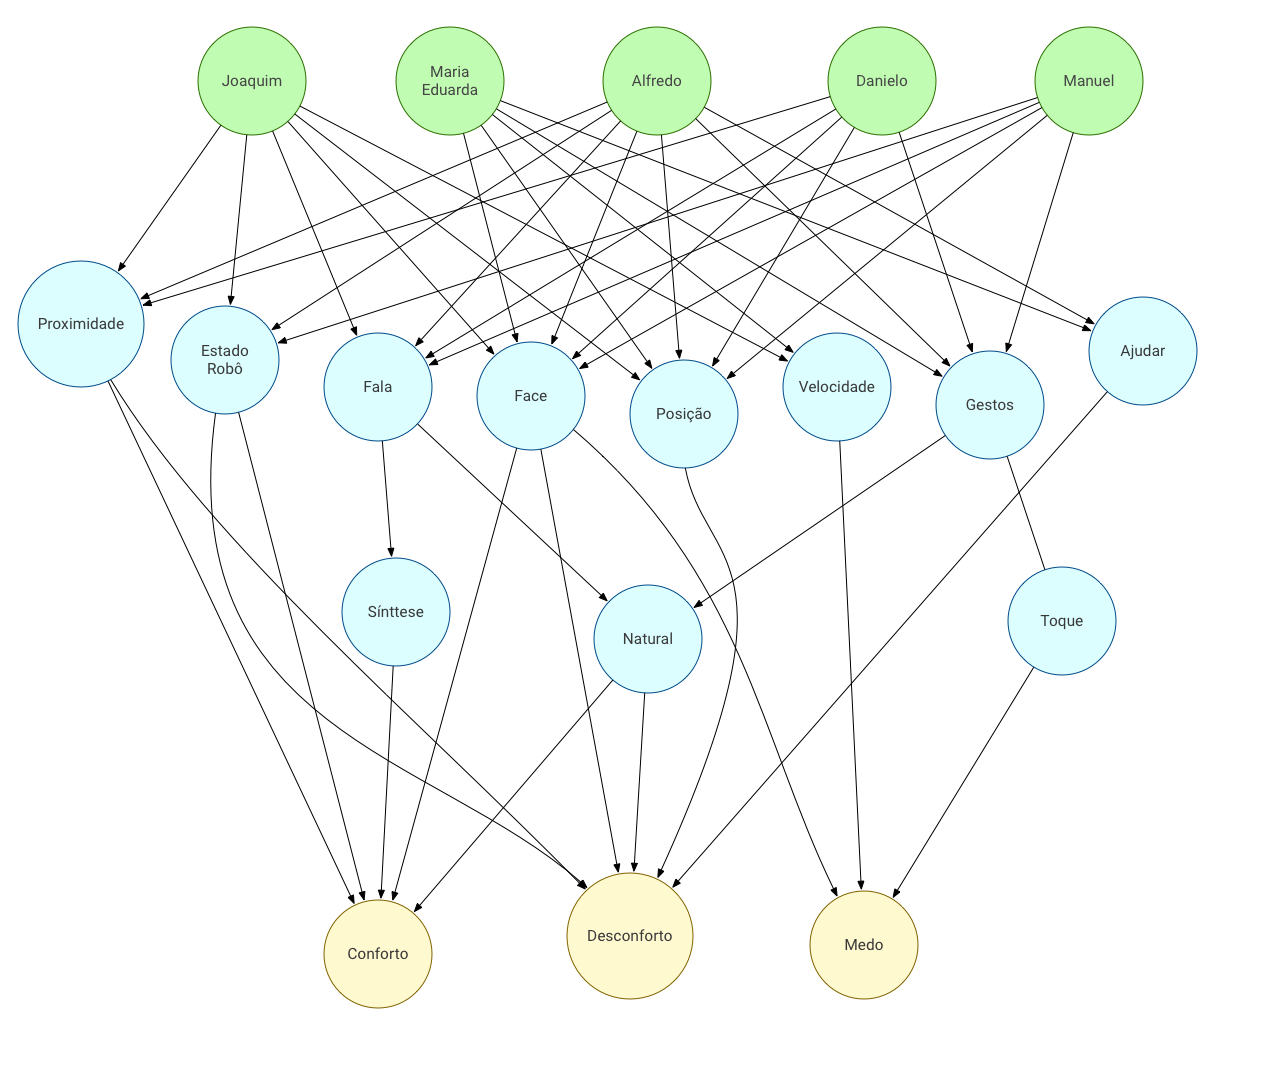
\includegraphics[width=\textwidth]{rb-thesis.png}
		\smallcaption{Fonte: Autor.}
		\label{fig:rb}
	\end{minipage}
\end{figure}

É importante ressaltar que a classificação do usuário é feita com base em sua experiência, pois é o principal interessado na interação com o robô. A grande preocupação em manter o foco no ser humano é por que ele é o mais interassado na interação com o sistema, já que irá conviver com o robô em sua casa brevemente. A tomada de decisão para melhorar a experiência do usuário a partir da classificação do perfil do usuário pelo robô não faz parte do escopo desta tese. Entretanto, uma lista com possíveis características a serem consideradas é apresentada na seção~\ref{sec:extracaocaracteristicas}. As variáveis para auxiliar melhor a identificação de características da interação podem complementar a camada interna da rede bayesiana e por consequência aprimorar os resultados do classificador bayesiano.
